%%%%%%%%%%%%%%%%%%%%%%%%%%%%%%%%%%%%%%%%%
% Wenneker Article
% LaTeX Template
% Version 2.0 (28/2/17)
%
% This template was downloaded from:
% http://www.LaTeXTemplates.com
%
% License:
% CC BY-NC-SA 3.0 (http://creativecommons.org/licenses/by-nc-sa/3.0/)
%
%%%%%%%%%%%%%%%%%%%%%%%%%%%%%%%%%%%%%%%%%

%----------------------------------------------------------------------------------------
%	PACKAGES AND OTHER DOCUMENT CONFIGURATIONS
%----------------------------------------------------------------------------------------

\documentclass[10pt, a4paper, twocolumn]{article} % 10pt font size (11 and 12 also possible), A4 paper (letterpaper for US letter) and two column layout (remove for one column)

%%%%%%%%%%%%%%%%%%%%%%%%%%%%%%%%%%%%%%%%%
% Wenneker Article
% Structure Specification File
% Version 1.0 (28/2/17)
%
% This file originates from:
% http://www.LaTeXTemplates.com
%
% Authors:
% Frits Wenneker
% Vel (vel@LaTeXTemplates.com)
%
% License:
% CC BY-NC-SA 3.0 (http://creativecommons.org/licenses/by-nc-sa/3.0/)
%
%%%%%%%%%%%%%%%%%%%%%%%%%%%%%%%%%%%%%%%%%

%----------------------------------------------------------------------------------------
%	PACKAGES AND OTHER DOCUMENT CONFIGURATIONS
%----------------------------------------------------------------------------------------

\usepackage[english]{babel} % English language hyphenation

\usepackage{microtype} % Better typography

\usepackage{amsmath,amsfonts,amsthm} % Math packages for equations

\usepackage[svgnames]{xcolor} % Enabling colors by their 'svgnames'

\usepackage[hang, small, labelfont=bf, up, textfont=it]{caption} % Custom captions under/above tables and figures

\usepackage{booktabs} % Horizontal rules in tables

\usepackage{lastpage} % Used to determine the number of pages in the document (for "Page X of Total")

\usepackage{graphicx} % Required for adding images

\usepackage{enumitem} % Required for customising lists
\setlist{noitemsep} % Remove spacing between bullet/numbered list elements

\usepackage{sectsty} % Enables custom section titles
\allsectionsfont{\usefont{OT1}{phv}{b}{n}} % Change the font of all section commands (Helvetica)

\usepackage[hidelinks,
			colorlinks=true,
			linkcolor=black,
			citecolor=blue,
			urlcolor=blue]{hyperref}

\usepackage{graphicx}
\graphicspath{ {./img/} }

\usepackage{xcolor}

\usepackage[toc,page]{appendix}

%----------------------------------------------------------------------------------------
%	MARGINS AND SPACING
%----------------------------------------------------------------------------------------

\usepackage{geometry} % Required for adjusting page dimensions

\geometry{
	top=1cm, % Top margin
	bottom=1.5cm, % Bottom margin
	left=2cm, % Left margin
	right=2cm, % Right margin
	includehead, % Include space for a header
	includefoot, % Include space for a footer
	%showframe, % Uncomment to show how the type block is set on the page
}

\setlength{\columnsep}{7mm} % Column separation width

\setlength\parindent{0pt} % No intent on new paragraphs

\renewcommand{\baselinestretch}{1.2} % Line spacing

%----------------------------------------------------------------------------------------
%	FONTS
%----------------------------------------------------------------------------------------

\usepackage[T1]{fontenc} % Output font encoding for international characters
\usepackage[utf8]{inputenc} % Required for inputting international characters

\usepackage{XCharter} % Use the XCharter font

%----------------------------------------------------------------------------------------
%	HEADERS AND FOOTERS
%----------------------------------------------------------------------------------------

\usepackage{fancyhdr} % Needed to define custom headers/footers
\pagestyle{fancy} % Enables the custom headers/footers

\renewcommand{\headrulewidth}{0.0pt} % No header rule
\renewcommand{\footrulewidth}{0.0pt} % Thin footer rule

\renewcommand{\sectionmark}[1]{\markboth{#1}{}} % Removes the section number from the header when \leftmark is used

%\nouppercase\leftmark % Add this to one of the lines below if you want a section title in the header/footer

% Headers
\lhead{} % Left header
% \chead{\textit{\thetitle}} % Center header - currently printing the article title
\rhead{} % Right header

% Footers
\lfoot{} % Left footer
\cfoot{} % Center footer
\rfoot{\footnotesize Page \thepage\ of \pageref{LastPage}} % Right footer, "Page 1 of 2"

\fancypagestyle{firstpage}{ % Page style for the first page with the title
	\fancyhf{}
	\renewcommand{\footrulewidth}{0pt} % Suppress footer rule
}

%----------------------------------------------------------------------------------------
%	TITLE SECTION
%----------------------------------------------------------------------------------------

\newcommand{\authorstyle}[1]{{\large\usefont{OT1}{phv}{b}{n}\color{Black}#1}} % Authors style (Helvetica)

\newcommand{\institution}[1]{{\footnotesize\usefont{OT1}{phv}{m}{sl}\color{Black}#1}} % Institutions style (Helvetica)

\usepackage{titling} % Allows custom title configuration

\newcommand{\HorRule}{\color{Gray}\rule{\linewidth}{1pt}} % Defines the gold horizontal rule around the title

\pretitle{
	\vspace{-30pt} % Move the entire title section up
	\HorRule\vspace{10pt} % Horizontal rule before the title
	\fontsize{22}{26}\usefont{OT1}{phv}{b}{n}\selectfont % Helvetica
	\color{DarkRed} % Text colour for the title and author(s)
}

\posttitle{\par\vskip 15pt} % Whitespace under the title

\preauthor{} % Anything that will appear before \author is printed

\postauthor{ % Anything that will appear after \author is printed
	\vspace{10pt} % Space before the rule
	\par\HorRule % Horizontal rule after the title
	\vspace{20pt} % Space after the title section
}

%----------------------------------------------------------------------------------------
%	ABSTRACT
%----------------------------------------------------------------------------------------

\usepackage{lettrine} % Package to accentuate the first letter of the text (lettrine)
\usepackage{fix-cm}	% Fixes the height of the lettrine

\newcommand{\initial}[1]{ % Defines the command and style for the lettrine
	\lettrine[lines=3,findent=4pt,nindent=0pt]{% Lettrine takes up 3 lines, the text to the right of it is indented 4pt and further indenting of lines 2+ is stopped
		\color{DarkGoldenrod}% Lettrine colour
		{#1}% The letter
	}{}%
}

\usepackage{xstring} % Required for string manipulation

\newcommand{\lettrineabstract}[1]{
	\StrLeft{#1}{1}[\firstletter] % Capture the first letter of the abstract for the lettrine
	\initial{\firstletter}\textbf{\StrGobbleLeft{#1}{1}} % Print the abstract with the first letter as a lettrine and the rest in bold
}

%----------------------------------------------------------------------------------------
%	BIBLIOGRAPHY
%----------------------------------------------------------------------------------------

\usepackage[backend=bibtex,style=authoryear,natbib=true]{biblatex} % Use the bibtex backend with the authoryear citation style (which resembles APA)

\addbibresource{example.bib} % The filename of the bibliography

\usepackage[autostyle=true]{csquotes} % Required to generate language-dependent quotes in the bibliography

\setlength\bibitemsep{4.0\itemsep}
 % Specifies the document structure and loads requires packages
\usepackage{subfiles} % Best loaded last in the preamble

\hyphenation{intersections OpenDataCam}

% Abstract type defination
\renewenvironment{abstract}
 {\small
  \begin{center}
  \bfseries\vspace{-.5em}\vspace{0pt}
  \end{center}
  \list{}{
    \setlength{\leftmargin}{3.0cm}%
    \setlength{\rightmargin}{\leftmargin}%
  }%
  \item\relax}
 {\endlist}


%----------------------------------------------------------------------------------------
%	ARTICLE INFORMATION
%----------------------------------------------------------------------------------------

\title{
	Quantifying cyclist behavior at intersections using automated video analysis 
	\ \\
	} % The article title

\author{
	\authorstyle{Edi Begovic and Høgni Jacobsen} % Authors
	\newline
	\institution{IT University of Copenhagen, Denmark}\\ % Institution
	\newline
	\authorstyle{Supervised by Michael Szell} % Authors
	\\ \\ \\
	
\includegraphics[width=3in]{img/ITUlogo} 
}

\date{\today} % Add a date here if you would like one to appear underneath the title block, use \today for the current date, leave empty for no date

%----------------------------------------------------------------------------------------
%	TITLE PAGE
%----------------------------------------------------------------------------------------

\begin{document}

\maketitle % Print the title
\thispagestyle{empty}  % Apply the page style for the first page (no headers and footers)

%----------------------------------------------------------------------------------------
%	ABSTRACT
%----------------------------------------------------------------------------------------

\twocolumn[\begin{@twocolumnfalse}
\ \\ \\
\begin{abstract}

\centerline{\LARGE \textbf{Abstract}} 

\ \\
In many European cities, such as Copenhagen and Amsterdam, cycling is an important part of urban 
transportation. But transport infrastructure often prioritizes cars, resulting in unfriendly or even dangerous 
environments for cycling. 
Having quantifiable data on the movement and behavior of cyclists is a crucial element in modern city B
planning and would result in friendlier urban infrastructure for cyclists. The current methods of dataB
collection are reliant on the human annotation of video recordings, which is expensive, time-consuming,B
and could face challenges in reproducibility. Here we set up and evaluate a new methodological approach to replace 
manual annotation.
In this approach we set up a data collection and analysis pipeline, consisting of camera selection and setup, 
video syncing, camera calibration, machine-learning based object detection, projection, merging of different 
camera sources, and object tracking. We also develop a web app for efficiently exploring collected footage. 
To test our setup in a case study, we record and analyze videos of the Dybbelsbro intersection in Copenhagen 
with multipe cameras. Our method succeeds to detect cyclist trajectories and to transform them into a 
birds-eye view, allowing us to explore both fine-grained details and an aggregated view of cyclist behavior.
Using our method we produce favorable results compared to manual annotation.

\end{abstract}
\end{@twocolumnfalse}]
\thispagestyle{empty}
\clearpage

%----------------------------------------------------------------------------------------
%	Table of Contents 
%----------------------------------------------------------------------------------------
\twocolumn[\begin{@twocolumnfalse}
\setcounter{tocdepth}{3} % Set the depth of the table of contents to show sections and subsections only
\tableofcontents % Print the table of contents
\end{@twocolumnfalse}]
\thispagestyle{empty}
\clearpage
%----------------------------------------------------------------------------------------
%	ARTICLE CONTENTS
%----------------------------------------------------------------------------------------

% Page numbering starts from here
\setcounter{page}{1}

\section{Introduction}
\subfile{sections/introduction}

\section{Background}
\subfile{sections/background}

\section{Methodological proposal}
\subfile{sections/proposal}

\section{Implementation}
\subfile{sections/methodology}

\section{Case studies}
\subfile{sections/results}

\section{Discussion}
\subfile{sections/discussion}

\section{Conclusion}
\subfile{sections/conclusion}

%----------------------------------------------------------------------------------------
%	BIBLIOGRAPHY
%----------------------------------------------------------------------------------------
\clearpage
\printbibliography[title={Bibliography}] % Print the bibliography, section title in curly brackets


%----------------------------------------------------------------------------------------
%   APPENDIX
%----------------------------------------------------------------------------------------

\onecolumn

\begin{appendices}
\section{Behavior analysis}
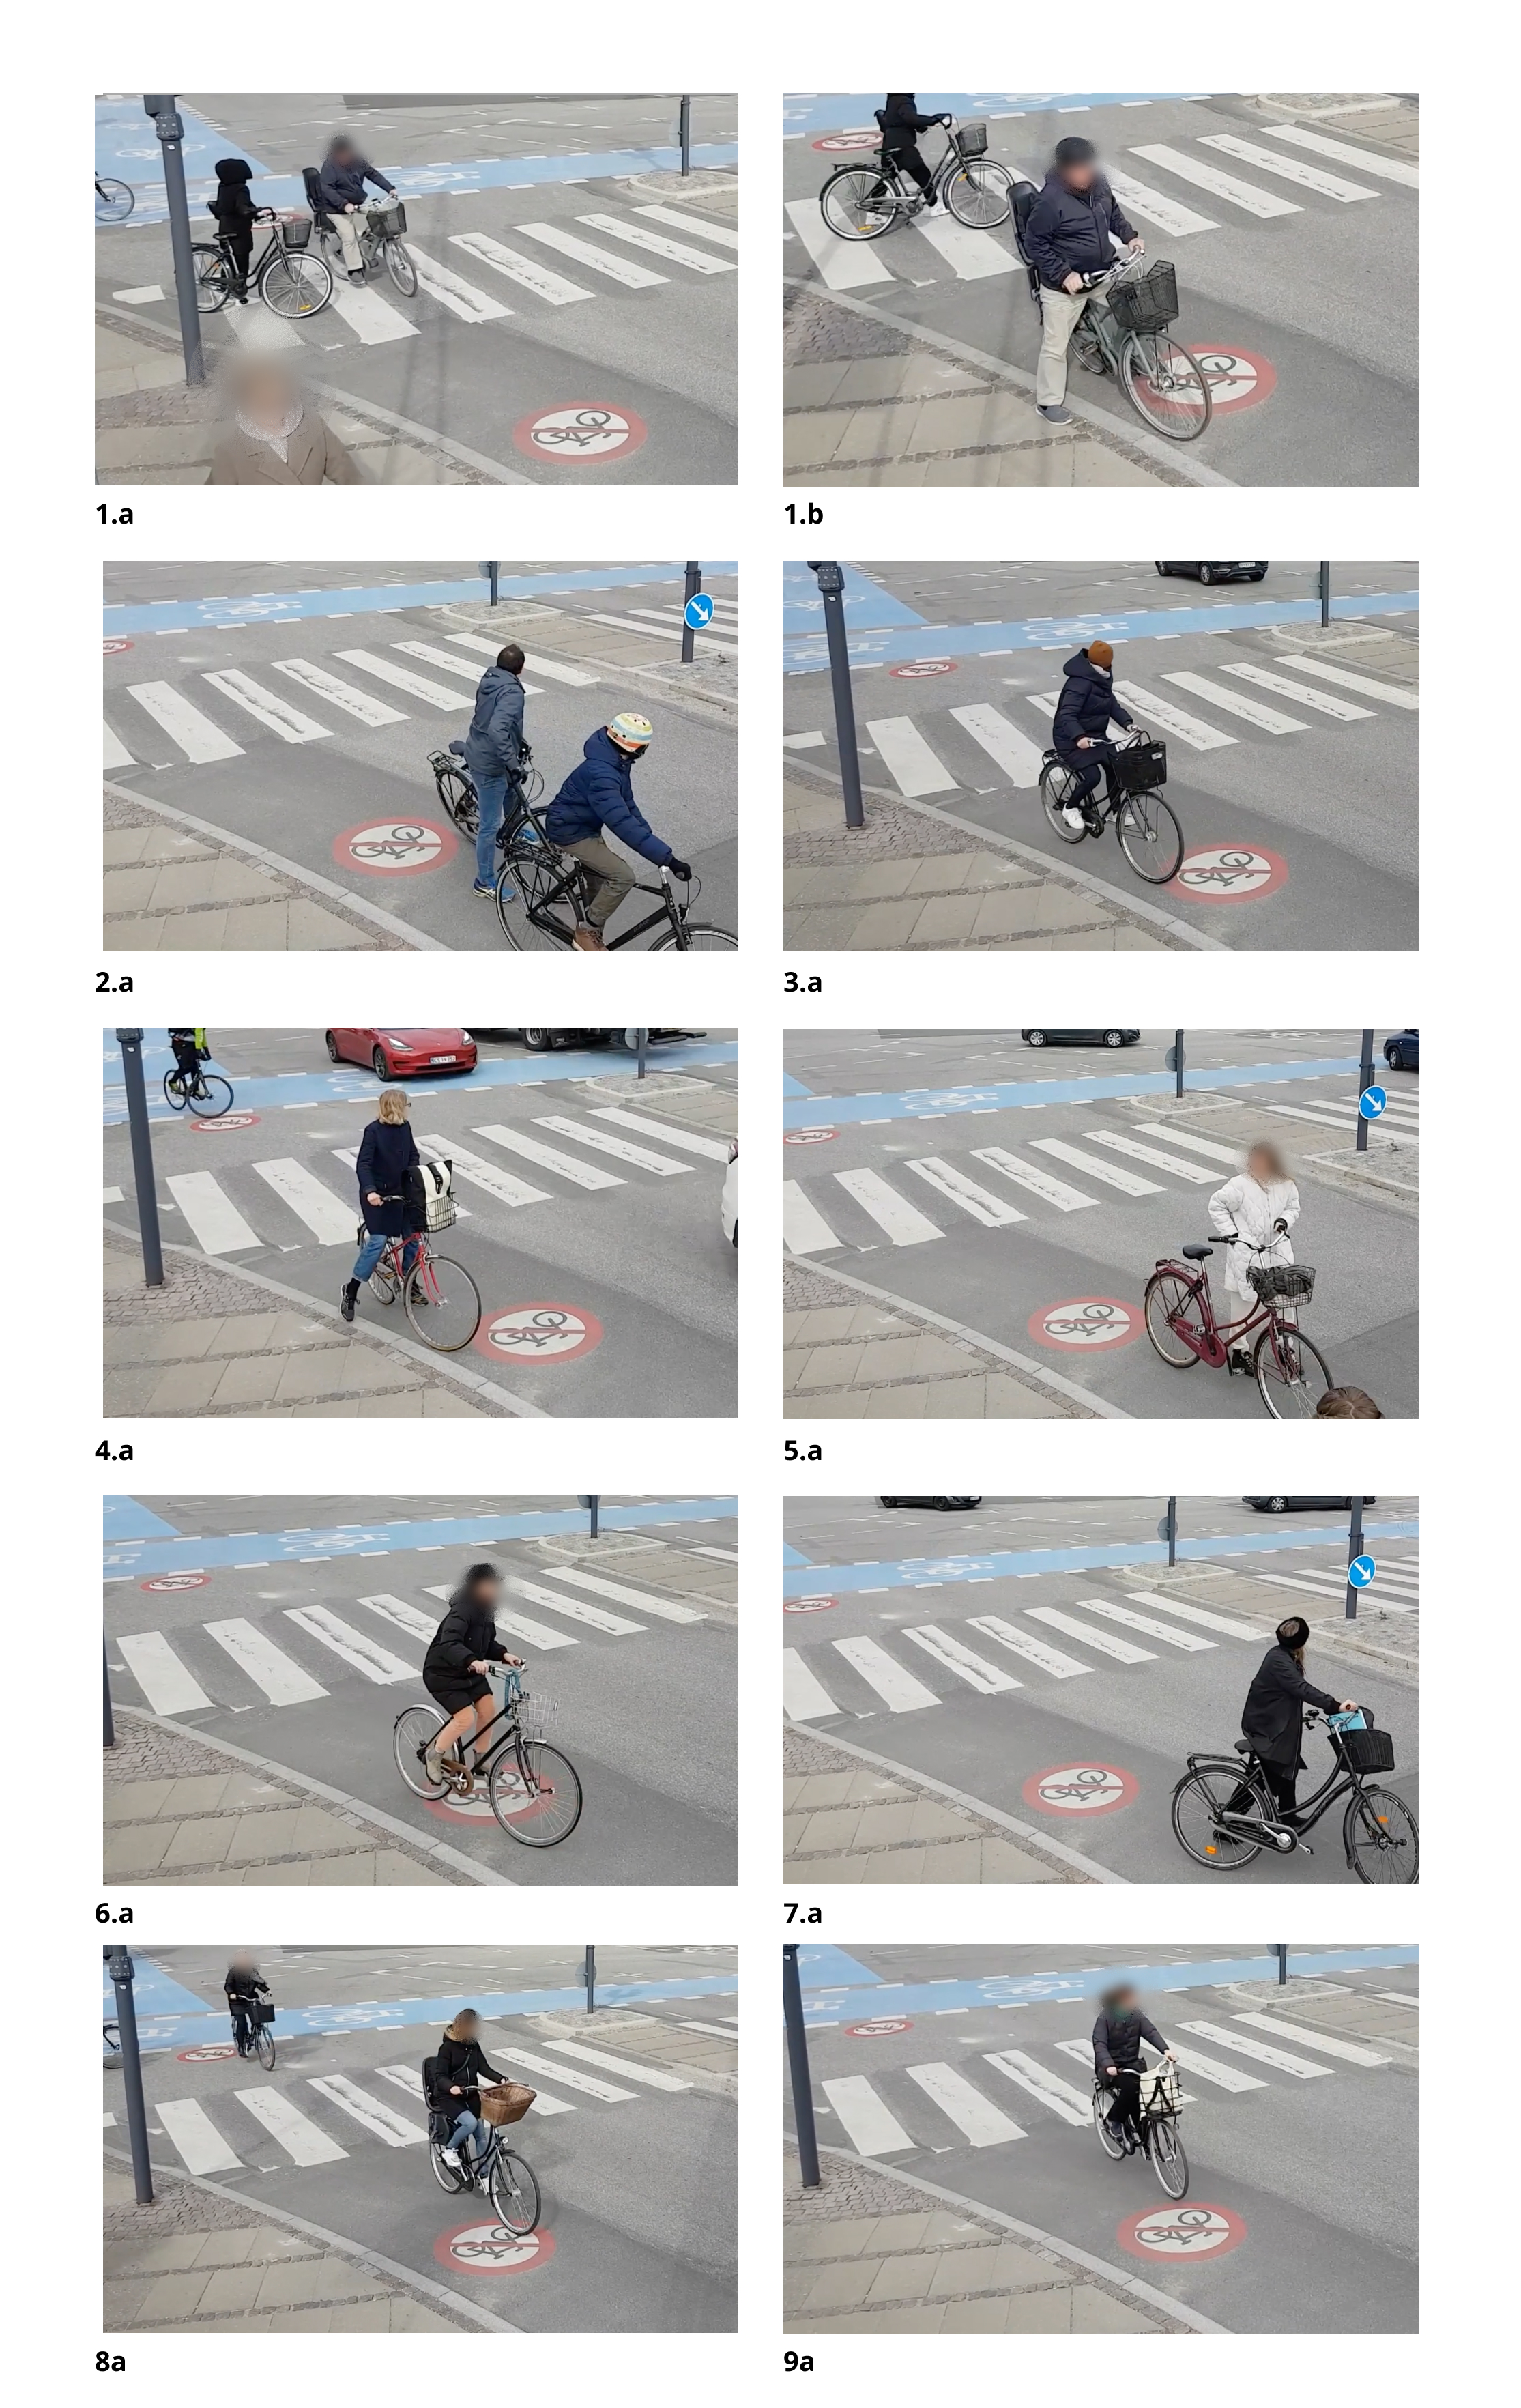
\includegraphics[scale=0.2]{confused.jpg} 

\end{appendices}

% ---------------------------------------------------------------------------------------
\end{document}